\documentclass{masterthesis}

\usepackage[
    pdftex,
    pdftitle={Learning relational models from networked data on the web},
    pdflang={en}
]{hyperref}
\usepackage{cmap}
\usepackage{graphicx}
\usepackage{enumitem}
\usepackage{amsmath}
\usepackage{mathtools}
\usepackage{float}
\usepackage{amssymb}
\usepackage{multicol}
\usepackage{dirtytalk}
\usepackage{subfigure}
\usepackage{bbold}
\usepackage{minted}
\usepackage[english]{babel}

\setminted{frame=lines, linenos}

\DeclareMathOperator*{\E}{\mathbb{E}}
\setlist[itemize]{topsep=0pt}
\setlist[enumerate]{topsep=0pt, itemsep=0pt}

\begin{document}

\title{Learning relational models \\ from networked data on the web}

\author{Davide Riva}

\advisor{Annalisa Barla, Davide Garbarino}

\examiner{Nicoletta Noceti}

\maketitle

\begin{abstract}
    \begin{center}
        
\includegraphics[width=0.5\textwidth]{images/meme.jpg}
    \end{center}
\end{abstract}

\dedication{
    I wish to express my deepest gratitude to all students and professors
    who went along with me on this journey.
    Among those, a special thanks to Eros Viola,
    Riccardo Bianchini, Olga Matthiopoulou, Marco Rando,
    Andrea Canepa, Larbi Touijer, Federico Lodovici,
    Roberto Castellotti, Antonio Vivace,
    Marco Orsingher, Michele Pugno,
    Annalisa Barla, Nicoleta Noceti and Davide Garbarino.

    In addition, I would like to thank Jordan Boyd-Graber and
    David M. Blei who released for free their lessons, talks and material
    which were useful during the writing of this thesis.

    I am also indebted to Fabio Antonio Stella,
    which made me fall in love with this subject
    and played an important role in the choices I made that led me here.

    I wish to acknowledge the support and great love of Laura
    and her family, which helped me tackle this degree course which is going to end.

    Last but not least,
    I would like to recognize the invaluable economic assistance
    that my family provided during my study.

    Thank you all.
}

\setcounter{tocdepth}{1}
\tableofcontents

\chapter{Introduction and motivation}
\dots

\chapter{Word Embedding} \label{wordemb}
Documents are made by words.
To be manipulable by an algorithm these words need to be represented in a numerical format.

This chapter covers some techniques able to fulfil this task,
pointing out the advantages and disadvantages of choosing one instead of another.

To avoid misunderstandings
we define the term \say{word} as a word in a particular position in a document,
while we use the word \say{term} as a generic word into a dictionary.

For instance, given a document \say{A cat is an animal but an animal is not a cat} its list of words
is $ w = (a, cat, is, an, animal, but, an, animal, is, not, a, cat)$
while its set of terms is $d = \{a, cat, is, an, animal, but, not\}$.

\section{One Hot Encoding}
Given a list of words $w = (w_1, w_2, \dots, w_N)$,
we first generate a dictionary of unique words
$d = \{d_1, d_2, ..., d_K\}$ with an arbitrary order between words.
Note that $ K \leq N $ is always true and $ K = N $ happens only when there is no repetition of words in the documents.

Each term $d_i$ in the dictionary can now be encoded as $x_i \in \{0,1\}^K$ following the One Hot Encoding approach.
All elements of $x_i$ are zero except a \say{1} in the position  $i$ of the vector.
That means that two words $w_l, w_j$ in different positions will have the same value $x_i$ if and only if they correspond to the same term $d_i$.

Applying One Hot Encoding on the previous example presented in the introduction of this chapter leads to the following values of $x_i$:
\begin{multicols}{2}
    \begin{itemize}
        \item $x_1 = x_{a} = [1, 0, 0, 0, 0, 0, 0]$
        \item $x_2 = x_{cat} = [0, 1, 0, 0, 0, 0, 0]$
        \item $x_3 = x_{is} = [0, 0, 1, 0, 0, 0, 0]$
        \item $x_4 = x_{an} = [0, 0, 0, 1, 0, 0, 0]$
        \item $x_5 = x_{animal} = [0, 0, 0, 0, 1, 0, 0]$
        \item $x_6 = x_{but} = [0, 0, 0, 0, 0, 1, 0]$
        \item $x_7 = x_{not} = [0, 0, 0, 0, 0, 0, 1]$
    \end{itemize}
\end{multicols}

Despite its simplicity and the fact that it is not computationally expensive to use, it has some disadvantages:
\begin{itemize}
    \item vectors are sparse: only one element of each vector is not zero
    \item there is no concept of similarity: all vectors have the same distance between each other
\end{itemize}

\section{Word2vec}

Word2vec is a family of approaches to overcome the disadvantages of One Hot Encoding using neural networks.
In this section, two architectures are proposed.
Both of them should be trained using mini-batch gradient descent instead of gradient descent to allow the algorithm to scale when datasets grow in size.

After a learning phase, they will be able to map each term $x_i \in \{0, 1\}^K$ to a point $y_i \in \mathbb{R}^V$, with $V \ll K$.
Points in the new space will have a notion of similarity:
if two terms $l$ and $j$ appear in similar contexts and/or they have the same semantic content,
their vectors $y_l$ and $y_j$ will be close together.
On the opposite situation, $y_l$ and $y_j$ will be distant from each other.

For instance, $y_{cat}$ will probably be more close to $y_{dog}$ than $y_{computer}$.

\subsection{Continuous Bag-of-Words Model (CBOW)}
First, the entire corpus is divided into contiguous blocks of words with odd length $N$ called n-grams.

Suppose to have the phrase \say{A cat is the best animal.} and n-grams of size $3$.
The corresponding blocks are:
\begin{multicols}{2}
    \begin{itemize}
        \item $(a, cat, is)$
        \item $(cat, is, the)$
        \item $(is, the, best)$
        \item $(the, best, animal)$
    \end{itemize}
\end{multicols}

The goal is to predict a word given its context.
For each n-gram, the CBOW neural network has as inputs all words in the block
except the one in the center which is used as ground truth for the classification task.
All words are encoded using the One Hot Encoding method.

For each n-gram, the first layer takes each input word encoded as $x_i \in \{0, 1\}^K$ and project it into a smaller space $\mathbb{R}^V$
where $V$ is a hyperparameter to tune.
This is done through a shared matrix $M_{K \times V}$ which represents a fully connected layer.
Each projection is then averaged out with the others in the same block.
Note that in this way the order of the input words of the same sequence does not matter anymore.

The previous layer is then linked to a final layer in a fully connected way.
Since the classification task is on a One Hot Encoding vector,
a softmax activation function is used at the end.

Instead of using the network for the task for which it was trained, we use the matrix $M_{K \times V}$ to encode all terms as vectors in $\mathbb{R}^V$.

Note that there is no need to compute $M x_i$ for each $i$.
Since every $x_i$ has zero values everywhere except a \say{1} in the position $i$ of the vector, the result of the multiplication $M x_i$ is the row $i$ of the matrix M.
For this reason, each row $i$ of $M$ represents the term in position $i$ of the dictionary, encoded using CBOW.

\subsection{Continuous Skip-gram Model (Skip-gram)}
The Skip-gram model is the opposite approach of CBOW.

For each n-gram, the word in the center is fed to the neural network as the only input.

The second layer projects it to a smaller space through a matrix $M_{K \times V}$.
Unlike the previous model, there is no averaging since there is just one word as input.

Finally, the last layer tries to predict all remaining words of a block.
Each predicted word is obtained multiplying the hidden layer with a shared matrix $M'_{V \times K}$.
For each group of $K$ nodes which refers to a predicted word we apply separately a softmax function.
To increase the accuracy, we can pick a number of output words less than $N-1$ and then sampling
words in the same phrase weighted by how distant they are from the input word.

If there are $N-1$ words to predict and each word is represented as a vector in $\mathbb{R}^K$,
the total number of nodes of the final layer is $(N-1)K$.

As previously, we use the matrix $M$ to encode each term $x_i$.

\subsection{Interpretation of the results}
The concept used in the previous method is similar to Autoencoders,
but in this scenario we are using the intermediate representation to predict words in the same phrase.
This leads to words that appear in the same context having close values of $y$.

Furthermore, the paper \cite{DBLP:journals/corr/abs-1301-3781}
found out these models go beyond syntactic regularities: for intance,
the operation $y_{king} - y_{man} + y_{woman}$ is closest to $y_{queen}$.
Note that subsequent papers like \cite{nissim2019fair} scale down the previous claim,
adding the constraint that no input vector can be returned by the prediction.

\section{Global Vectors for Word Representation (GloVe)}
\dots
\chapter{Topic Modeling}

In Chapter \ref{wordemb}, we presented some techniques to encode words as vectors.
Starting from a bag-of-words model in which we assume that the order of the words
inside a text does not matter, it is possible to follow a similar approach also for documents.

The first step is to generate a matrix of term counts $X$ for the entire corpus:
each row is a document represented in the BOW format and each column represents the count of occurrence
of a particular term in the documents.

The goal of the second step is to produce two matrices:
\begin{itemize}
    \item term-topic matrix: each row represents how related each term is to all topics
    \item document-topic matrix: each row represents how related each document is to all topics
\end{itemize}

For instance, a document about bears is likely to have high intensity on some topics which in turn have high
intensity on words related to animals.

\section{Latent Semantic Analysis (LSA)}
Given the number of topics $V$ as an hyperparameter,
Truncated SVD is applied to the matrix obtained in the first step:
$$X_{N \times K} = U_{N \times V} \Sigma_{V \times V} D_{K \times V}^T$$

The matrix $U$ is then used as the document-topic matrix,
while $D$ represents the term-topic matrix.

Using $U$ instead of $X$ for comparing documents when $V \ll K$ leads to a smaller memory footprint.
Furthermore, the terms are no longer orthogonal: thanks to this it is possible to compute the similarity between
a term and a document even if the document does not contain the term itself.
The key point to observe is that both terms and documents are described as topics: if a term is frequent in some topics and
a document is frequent in the same topics, they will have a similar representation in the new space.

An overview of this technique can be found at \cite{doi:10.1002/aris.1440380105}.

\section{Latent Dirichlet Allocation (LDA)}
\dots

\section{Hierarchical Dirichlet Process (HDA)}
\dots
\chapter{Network inference}

Network inference is the process of inferring a set of links among variables
that describe the relationships between data.
In particular, in this chapter, we describe ARACNE, an algorithm introduced by \cite{DBLP:journals/bmcbi/MargolinNBWSFC06}
for the reconstruction of Gene Regulatory Networks (GRNs).

\section{ARACNE} \label{aracne}
ARACNE (Algorithm for the Reconstruction of Accurate Cellular Network)
can describe the interactions in cellular networks
starting from microarray expression profiles;
the result is an undirected graph of the regulatory influences between genes.

This type of method arises from the need of having tools to separate artifacts
from real gene interactions.
In particular, ARACNE can be divided into three steps:
\begin{enumerate}
    \item computation of Mutual Information (MI) between genes
    \item identification of a meaningful threshold
    \item Data Processing Inequality (DPI)
\end{enumerate}

\subsection{Computation of Mutual Information (MI) between genes} \label{MI}
Mutual Information is a measure of relatedness between two random variables.
For two discrete variables $x$ and $y$, it is defined as:
\[ \mathit{MI}(x, y) = H(x) + H(y) - C(x, y) \]
where $H(x)$ is the entropy of $x$ and $C(x, y)$ is the joint entropy between $x$ and $y$.
Note that from the definition of Mutual Information,
$\mathit{MI}(x, y) = 0$
if and only if $P(x, y) = P(x) P(y)$.

In our case, for each combination of genes $x, y$ with $M$ observations we want to obtain:
\[ \mathit{MI}(\{ x_i \}_{i=1,\dots,M}, \{ y_i \}_{i=1,\dots,M}) \]
Since microarray data is expressed by continuous variables,
we have to use the differential entropy instead of the entropy
and the joint differential entropy instead of the joint entropy.
For this reason, an estimation of $p(x)$
using Kernel Density Estimation (KDE) is first needed:
\[ \hat{p}(x) = \frac{1}{M} \sum_{i=1}^{M} K(x - x_i) \]
where $i$ is an index which iterates through all observations of a gene $x$
and $K(.)$ is a kernel.
In particular, \cite{DBLP:journals/bmcbi/MargolinNBWSFC06} proposes
$K(.)$ to be a Gaussian kernel.

Finally, we compute the MI between two genes $x, y$ using the formula:
\begin{align*}
    \mathit{MI}(\{ x_i \}, \{ y_i \}) & = \iint \hat{p}(x, y) \log [\frac{\hat{p}(x, y)}{\hat{p}(x) \hat{p}(y)}] \, dx \, dy          \\
                                      & \approx \frac{1}{M} \sum_{i=1}^{M} \log [\frac{\hat{p}(x_i, y_i)}{\hat{p}(x_i) \hat{p}(y_i)}]
\end{align*}

\subsection{Identification of a meaningful threshold} \label{threshold-aracne}
Since the MI can not be zero by construction
and there might be spurious dependencies between genes,
we now want to find a threshold for which
all pairs of genes with a MI under that value are considered independent.

To do so, we first randomly shuffle the expression of genes for each observation
and we then compute the MI using this new dataset.
This process is repeated several times,
to obtain an approximate distribution of MIs under the condition of shuffled data.

We then set a p-value $p$, assuming that the first $1-p$ percentage of
MIs in the distribution of shuffled data is random noise.
We then identify the biggest MI value in that group to be used as a threshold.

Given the MI values obtained in Section \ref{MI},
we now set to zero the ones lower than the threshold.

\subsection{Data Processing Inequality (DPI)}
Finally, the DPI step prunes indirect relationships for which two
genes are co-regulated by a third one but their MI is nonzero.

Given each possible triplet of genes $(x, y, z)$,
it checks if $\mathit{MI}(x, z) \leq \min[\mathit{MI}(x, y), \mathit{MI}(y, z)]$
and in that case it sets $\mathit{MI}(x, z) = 0$.

At the end, two genes are connected by an undirected link if and only if
their final MI is greater than zero.
\chapter{Experiments}
Introduction here

\section{Crawling}
In order to collect data, we selected some monolingual websites to experiment with (see Table \ref{table:dbinfo}).

Then, we implemented a spider (see Section \ref{spider}) to download and store all HTML documents in a particular domain.
The application can be summarized with these steps:
\begin{enumerate}[topsep=0pt, itemsep=0pt]
    \item first, the software starts from an URL defined by the user, putting it into a pool
    \item if the pool is not empty, the application will get a link from it, starting its download. After getting the link, it is removed from the pool
    \item if the content is a valid HTML document, it is stored
    \item all links of that webpage that are in the specified domain are stored. They are also put into the pool if they were not analyzed previously
    \item loop to step 2 until there are no links left
\end{enumerate}
The final result is a set of tuples \texttt{(url, connected\_to, content)}, where \texttt{url} is the URL of a particular page, \texttt{connected\_to} is its set of links and \texttt{content} is its HTML source code.
Scrapy allows saving these results in different formats, but we choose to save everything in CSV files in order to re-use them easily in the next phases.

To get an idea of the size of each dataset, we report the number of documents and the number of unique words in Table \ref{table:dbdata}.

\begin{table}[H]
    \resizebox{\columnwidth}{!}{
        \begin{tabular}{ |l|l|l|l|l| }
            \hline
            ID                & URL                                & Domain                & Language & Date of acquisition \\
            \hline
            \hline
            bnu               & https://english.bnu.edu.cn/        & english.bnu.edu.cn    & en       & 2020-03-06          \\
            \hline
            goop              & https://goop.com/                  & goop.com              & en       & 2020-03-03          \\
            \hline
            ilblogdellestelle & https://www.ilblogdellestelle.it/  & ilblogdellestelle.it  & it       & 2020-03-03          \\
            \hline
            ilpost            & https://www.ilpost.it              & ilpost.it             & it       & 2020-03-02          \\
            \hline
            msccrociere       & https://www.msccrociere.it/        & msccrociere.it        & it       & 2020-03-02          \\
            \hline
            postgraduate      & https://www.postgraduateforum.com/ & postgraduateforum.com & en       & 2020-03-03          \\
            \hline
            rottentomatoes    & https://www.rottentomatoes.com     & rottentomatoes.com    & en       & 2020-03-02          \\
            \hline
            watt              & https://www.wattpadwriters.com     & wattpadwriters.com    & en       & 2020-03-03          \\
            \hline
        \end{tabular}
    }
    \caption{List of websites crawled. Languages follow the ISO 639-1 format, while dates are represented according to ISO 8601.}
    \label{table:dbinfo}
\end{table}

\begin{table}[H]
    \begin{center}
        \begin{tabular}{ |l|l|l| }
            \hline
            ID                & N. of documents & N. of unique words \\
            \hline
            \hline
            bnu               & 1350            & 15044              \\
            \hline
            goop              & 25147           & 116082             \\
            \hline
            ilblogdellestelle & 27190           & 132650             \\
            \hline
            ilpost            & 729372          & 459936             \\
            \hline
            msccrociere       & 530             & 21284              \\
            \hline
            postgraduate      & 48690           & 114730             \\
            \hline
            rottentomatoes    & 84740           & 240916             \\
            \hline
            watt              & 492             & 18060              \\
            \hline
        \end{tabular}
    \end{center}
    \caption{The number of documents and unique words for each dataset obtained during the crawling phase.}
    \label{table:dbdata}
\end{table}
\chapter{Conclusions and future work} \label{conclusions}
The main purpose of this work was to infer
 similarities between documents in a collection,
obtaining a network in which vertices are documents and
edges express similarities of the content.
In particular, we worked with scraped websites
showing that for our data it is possible to construct
a graph of relations between thousands of webpages
without scaling issues. 
Note that being a website is not a requirement and 
our pipeline can be used in the future also for 
datasets which are only a collection of documents.

An extension of our pipeline might be to consider the semantic tags, 
assigning different weights to the text inside them. 
An example could be to consider each title inside a \say{\textless h1\textgreater} 
tag twice important than text outside it, 
counting the words twice during the Bag-of-Words conversion.

Due to limited time, we dealt with monolingual
websites, but we propose an approach to overcome this issue.
The problem can be divided into two steps:
an automatic identification of the language of a portion of text and
the production of an algorithm to have the same Bag-of-Words
representation for each concept expressed in different languages.
Since we are working with web data, it is possible to retrieve the language
of the content of each webpage by looking at the Content-Language entity header
(see \cite{rfc7231}) or the lang global attribute
(see the HTML 5.1 W3C Recommendation\footnote{\url{https://www.w3.org/TR/html51/dom.html\#the-lang-and-xmllang-attributes}}).
Note that the second approach is preferable when \say{lang} is provided
since it handles the situation in which at least
one webpage is composed of sections with different languages.
When both options are not available,
a language identification model
(see fastText resources\footnote{\url{https://fasttext.cc/docs/en/language-identification.html}})
could be used as a failover.
In order to have different languages with a common Bag-of-Words
representation, we could translate each document to a pre-defined language
and then compute the BoW format for each document as previously done.
The lack of pre-trained models covering a wide range
of languages requires to find alternative solutions to the problem of translation.
we suggest to look for already trained multilingual word embeddings
which are aligned in a common space (see fastText resources\footnote{\url{https://fasttext.cc/docs/en/english-vectors.html}})
to use them to find an association between words expressing the same concept in different languages.
The assumption we made in the last scenario is that words in different languages share
the same meaning and for this reason different word vectors of different languages differ only on the basis
of the vector space in which they are represented.
The interested reader may refer to \cite{DBLP:journals/corr/abs-1804-07745} for further analysis of the topic.

Preliminary results suggest that the inferred network can 
model relations between topics. 
Further analyses could be made with different datasets in order to 
empirically verify what we observed with our data. 
In particular, we propose Cora\footnote{\url{https://linqs.soe.ucsc.edu/data}} 
since it provides a network of connections between documents that can be used as 
a ground truth.

\appendix
\chapter{Neural Networks}
The goal of this appendix is to give a simple albeit incomplete introduction of
Neural Networks for those readers who have not a solid background on it but
still they are interested in Chapter \ref{wordemb}.

\section{Gradient descent}
Given a minimization problem $min_w f(w), w \in \mathbb{R}^D$,
it is possible to find a local minimum through gradient descent.

First, we compute the gradient $\nabla f(w)$ and we decide a point $w_0$ in which the algorithm has to start.
If the problem is not convex, choosing a different $x_0$ could lead to a different
solution.
Since gradients point in the direction of fastest increase,
we take small steps towards the opposite direction in order to reach a minimum.

The step size is controlled by a hyperparameter $\lambda$:
values too small for a particular problem increase
the time needed to obtain a good solution and
it can lead to a local minimum;
values too big prevent convergence.

The final equation is:
$$ w_{i+1} = w_{i} - \lambda \nabla f(w_i) $$

Each step is run iteratively until a stopping criterion is met.
If the algorithm is stopped after $I$ iterations, the solution
for the minimization problem is $w_{I}$.
Common sense stopping criterions could be:
\begin{itemize}
    \item stop after a prefixed number of iterations
    \item stop when the results are not getting better for the last $I$ steps
    \item stop when $f(w_i) - f(w_{i+1}) < \epsilon$, with $\epsilon > 0$ small
\end{itemize}

Note that the parameter $\lambda$ could be different at each iteration:
$$ w_{i+1} = w_{i} - \lambda_{i+1} \nabla f(w_i) $$
For instance, we could have $\lambda_i = \frac{\lambda}{i}$ in order to take
smaller and smaller steps until convergence.

\subsection{Gradient descent in action} \label{gradesc}
Suppose to have a dataset $X \in \mathbb{R}^{N \times D}, y \in \mathbb{R}^N$.

What we want to do is linear regression, whose model is obtained resolving:
$$\displaystyle \min_{w \in \mathbb{R}^D} \frac{1}{2N} \sum_i (w^T x_i - y_i)^2$$

The derivative  $\frac{1}{2N} \sum_i (w^T x_i - y_i)^2 dw$ is:
$$\frac{1}{2N} \sum_i 2 x_i(w^T x_i - y_i) = \frac{\sum_i x_i(w^T x_i - y_i)}{N}$$

Therefore:
$$ w_{n+1} = w_n - \frac{\lambda}{N} \sum_i x_i(w_i^T x_i - y_i) $$


\section{Mini-batch gradient descent}
There are situations in which using gradient descent is not computationally feasible.
For instance, imagine that the problem explained in Section \ref{gradesc} have
a number of points so huge that a solution can not be obtained in feasible times.

Mini-batch gradient descent is an extension of gradient descent which assume that
samples of $|M|$ elements of the dataset are a noisy representative of the entire data.
At each step, $M$ will be re-sampled from $X$.

In that case, the minimization presented in Section \ref{gradesc} can be rewritten as:
$$\displaystyle \min_{w \in \mathbb{R}^D} \frac{1}{2|M|} \sum_{x_i \in M} (w^T x_i - y_i)^2 $$

\section{Linear Neural Networks}
The linear regression exposed in Section \ref{gradesc} can be viewed as a Neural Network
which has $D$ inputs as a first layer and a single neuron as output connected to all previous ones.

The graphical representation of it can be see in PICTURE MIAO.

That the vector $w$ is simply the set of all weights.
Starting from the equation presented in Section \ref{gradesc}:
$$ w_{n+1} = w_n - \frac{\lambda}{N} \sum_i x_i(w^T x_i - y_i) $$
each weight $w_i$ can be parallely updated:
$$ w_{(n+1)j} = w_{nj} -  \frac{\lambda}{N} \sum_i x_{ij}(w^T_j x_{ij} - y_i) $$

In this example the cost function is the square loss, but there is not any particular requirement when
dealing with Neural Networks.

\section{Activation functions}
For each node, a non-linear function could be applied before moving the output to the next layer.
For the sake of simplicity, we are going to present a model similar to the previous one,
with the difference that a $\tanh$ function is applied to the output node:
$$ \displaystyle \min_{w \in \mathbb{R}^D} \frac{1}{2N} \sum_i [\tanh(w^T x_i) - y_i]^2 $$

To use gradient descent, we have to apply the chain rule.
Since $\tanh(z) dz = 1 - tanh^2(z)$:
$$ \frac{1}{2N} \sum_i [\tanh(w^T x_i) - y_i]^2 dw =
    \frac{1}{2N} \cdot \sum_i 2[\tanh(w^T x_i) - y_i] \cdot [1 - tanh^2(w^T x_i)] \cdot x_i $$
$$ w_{n+1} = w_n -
    \frac{\lambda}{N} \sum_i [\tanh(w^T x_i) - y_i] [1 - tanh^2(w^T x_i)] x_i $$

Other activation functions can be used instead of $\tanh$.
The one used in the models presented in Chapter \ref{wordemb} is the softmax
$\sigma(z), z \in \mathbb{R}^V$:
$$\sigma(z, j) =  \frac{e^{z_i}}{\sum_j e^{z_j}}$$
$$ \sigma(z) =
    \begin{bmatrix}
        \sigma(z, 1) \\ \sigma(z, 2) \\ ... \\ \sigma(z, V)
    \end{bmatrix}
$$

\section{Multilayer Neural Networks}
Adding intermediate layers (usually referred as hidden layers in the literature)
to a linear Neural Network is useless
since the product of linear components is again linear.
As an example, construct a model which the following characteristics:
\begin{itemize}
    \item $X \in \mathbb{R}^{N \times 2}$: 2 nodes as input
    \item $y \in \mathbb{R}^N$: 1 node as output
    \item 2 nodes in the hidden layer, fully connected to the two other layers
\end{itemize}
Its graphical representation can be seen in Figure MIAOMIAO
and the relative minimization function is:
$$ \displaystyle \min_{M, w} \frac{1}{2N} \sum_i [ w(M x_i) - y_i)^2 ]
    \ \text{with} \
    M \in \mathbb{R}^{2 \times 2}, w \in \mathbb{R}^{2}$$
which is again linear regression, but more computationally expensive.

On the opposite, stacking more layers while using a non-linear activation function
leads to an enriched hypothesis space. Learning weights in a deep Neural Network
(a Neural Network with multiple hidden layers) require using the backpropagation algorithm.

\subsection{Chain rule}
The chain rule states that, given $\hat{y} = f(g(x))$ its derivative is:
$$ \frac{d\hat{y}}{dx} = \frac{f(g)}{dg} \cdot \frac{g(x)}{dx} $$

It can be seen as a Neural Network with one layer as input, one as output and one in the hidden layer.
Its graphical representation can be viewed in Figure MIAOMIAOOO.
\chapter{Probability distributions}
Over all probability distributions used in this document, some of them are not usually part of the canonical background of a computer scientist.
We decided to present them in this appendix in order to have an overview for who has never seen them before.

\section{Beta distribution} \label{betad}
The Beta distribution is a family of continuous probability distributions.
It is defined in the range $[0, 1]$ and it has two parameters $\alpha,\beta > 0$.

Since $\alpha$ and $\beta$ are concentration parameters, they induce more and more sparsity as they approach the value of zero.
If $\alpha = \beta = 1$, the probability density function is uniform over $[0, 1]$.
As their values grow, the distribution tightens over its expectation.
All these observations can be seen empirically in Figure \ref{fig:betaparams}.

Due to its characteristics, it is suited to model probabilistic outcomes (for example, to describe how confident we are about the fact that a coin is loaded or not).

\begin{figure}[h]
    \centering
    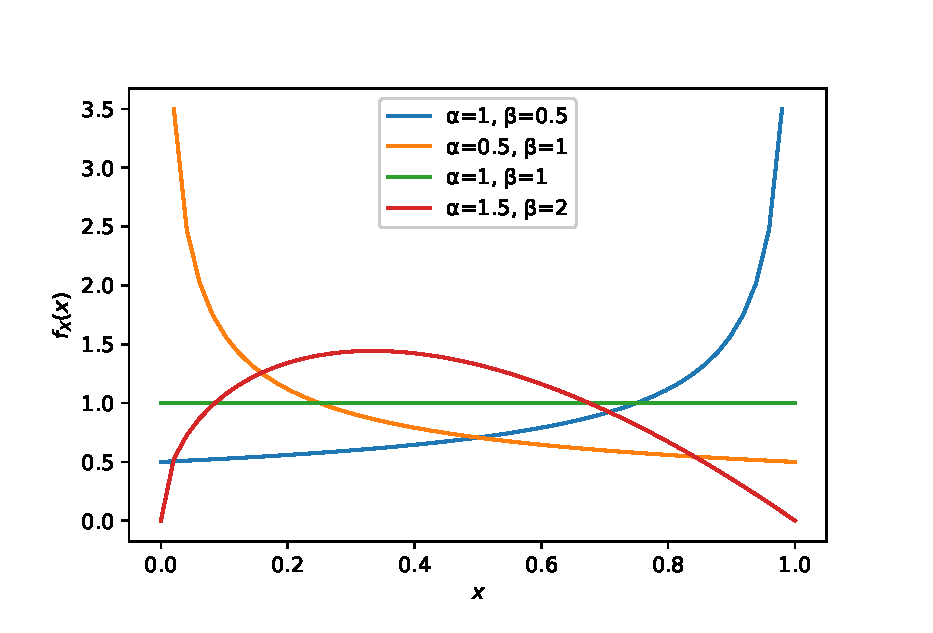
\includegraphics[width=0.7\textwidth]{images/beta}
    \caption{Example of the probability density function of a Beta distribution varying its parameters.}
    \label{fig:betaparams}
\end{figure}

\subsection{Probability density function}
Given a random variable $X \sim \mathit{Beta}(\alpha, \beta)$, the probability density function is defined as:
\[f_X(x) = \frac{1}{B(\alpha, \beta)}x^{\alpha - 1}(1-x)^{\beta - 1}\]
$\mathit{Beta}(\alpha, \beta)$ is the Beta function and it acts as a normalization constant to ensure that $\int_0^1 f_X(x) dx = 1$.

\section{Dirichlet distribution}
The Dirichlet distribution is a family of multivariate distributions.
It is parametrized by $K$ parameters, where $K$ is the number of random variables for which it is described.

It can be seen as a generalization of the Beta distribution: a Dirichlet distribution of 2 parameters $\mathit{Dir}(\alpha_1=a, \alpha_2=b)$ is a Beta distribution $\mathit{Beta}(\alpha=a, \beta=b)$.
All considerations and constraints about the parameters of the Beta distribution presented previously (Section \ref{betad}) still holds for the Dirichlet distribution.

\subsection{Probability density function}
Given a multivariate random variable $X \sim \mathit{Dir}(\alpha_1, \alpha_2, \dots, \alpha_K)$, the probability density function is defined as:

\[f_{X}(x_1, x_2, \dots, x_K; \alpha_1, \alpha_2, \dots, \alpha_K) = \frac{1}{B(\alpha_1, \alpha_2, \dots, \alpha_K)} \prod_{i=1}^{K} x_i^{\alpha_i - 1}\]

$\mathit{Beta}(\alpha_1, \alpha_2, \dots, \alpha_K)$ is the multivariate generalization of the Beta function presented in Section \ref{betad}.

Setting $\mathit{Dir}(\alpha) \coloneqq \mathit{Dir}(\alpha_1, \alpha_2, \dots, \alpha_n)$, a simplified notation of the probability density function is used:
\[f_{x}(x_1, x_2, \dots, x_K; \alpha) = \frac{1}{B(\alpha)} \prod_{i=1}^{K} x_i^{\alpha - 1}\]

The support is constrained by:
\begin{itemize}
    \item $x_i \in (0, 1), 1 \leq i \leq K $
    \item $\sum_{i=1}^K x_i = 1$
\end{itemize}

\subsection{Graphical intuition}
The support of a Dirichlet distribution with $K$ parameters lies in a $K-1$ simplex.
If $K=3$, the simplex is a triangle and can be represented graphically (see Figure \ref{fig:dirparams}).

All values of the probability density function $f_X(x_1, x_2, x_3): \Re^3 -> \Re$ are associated with a specific color given their intensity.
Bigger values in the probability density function are represented with lighter colors and vice versa.

Vertices of the simplex represent the situations in which $x = \begin{bmatrix}1 & 0 & 0 \end{bmatrix}$, $x = \begin{bmatrix}0 & 1 & 0 \end{bmatrix}$ or $x = \begin{bmatrix}0 & 0 & 1 \end{bmatrix}$.
If $x = \begin{bmatrix}\frac{1}{3} & \frac{1}{3} & \frac{1}{3} \end{bmatrix}$, we are at the center of the simplex.
Given an area of the triangle lighter than others, the probability of obtaining a vector in that interval during sampling is higher and vice versa.

Suppose we are in a supermarket and we are interested in the kind of purchases consumers make.
We define three categories: \say{food}, \say{technology} and \say{stationery}.
A strong preference over one category is represented modelling the probability density function with higher values towards one of the vertices.
Sampling from a Dirichlet distribution as the one represented in the left simplex in Figure \ref{fig:dirparams} will tend to give us users who do not have a strong preference over one category.
The opposite situation (for example, $\alpha_1=0.1, \, \alpha_2=0.1, \, \alpha_3=0.1$) will otherwise give us customers who strongly prefer one of the categories (for example. $x = \begin{bmatrix}0.8 & 0.15 & 0.05 \end{bmatrix}$) while users without propensities will be much rare.
Finally, if the probability density function is uniform over all the support (right simplex in Figure \ref{fig:dirparams}) there is no tendency of choosing a particular combination of categories over others.

\begin{figure}[h]
    \centering
    \subfigure{\includegraphics[width=0.5\textwidth]{images/Dirichlet-1}}%
    \hfill
    \subfigure{\includegraphics[width=0.5\textwidth]{images/Dirichlet-2}}
    \caption{Example of the probability density function over a simplex of a Dirichlet distribution varying its three parameters $\alpha = (\alpha_1, \alpha_2, \alpha_3)$. The lighter the color, the higher the probability density function.}
    \label{fig:dirparams}
\end{figure}

\section{Categorial distribution}
The categorical distribution is a generalized Bernoulli distribution in the case of categorical random variables.

In the literature about Topic Modeling, it is wrongly used with the name of Multinomial distribution.
To keep the same notation as the papers in the bibliography, we will say that $X \sim \mathit{Mult}(p)$ means that X is distributed as Categorical.
Note that a Categorical distribution $\mathit{Mult}(p)$ is a special case of a Multinomial distribution $\mathit{Mult}(n, p)$ in which $n=1$.

Each $p_i$ of the parameter $p = (p_1, p_2, \dots, p_K)$ represents the probability of observing $i$ by sampling from the distribution.

\subsection{Probability mass function}
Given a random variable $X \in \mathit{Mult}(p)$, the probability mass function is defined as:
\[P(x == i) = p_i\]

\section{References}
The interested reader may refer to \cite{Gupta2011}, \cite{DBLP:journals/jmlr/BleiNJ03} and \cite{Seber2011} to use them as references.
\chapter{Probability distributions closeness}
Some methods were developed to assess closeness between different probability distributions (see Figure \ref{fig:diffkl}).

In this appendix, we cover the ones which are used in the thesis.

\begin{figure}[h]
    \centering
    \subfigure{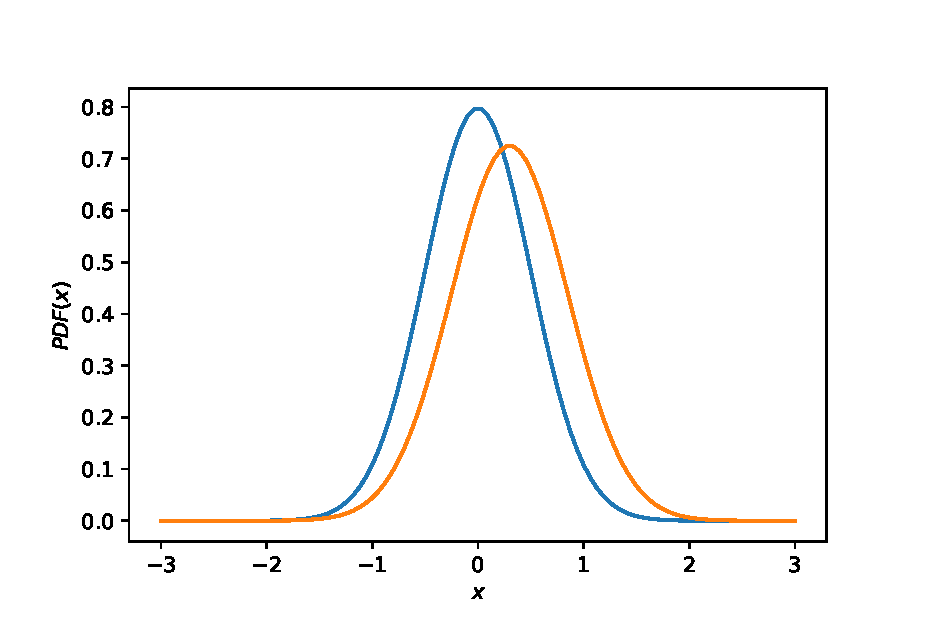
\includegraphics[width=0.5\textwidth]{images/diff-kl-1}}%
    \hfill
    \subfigure{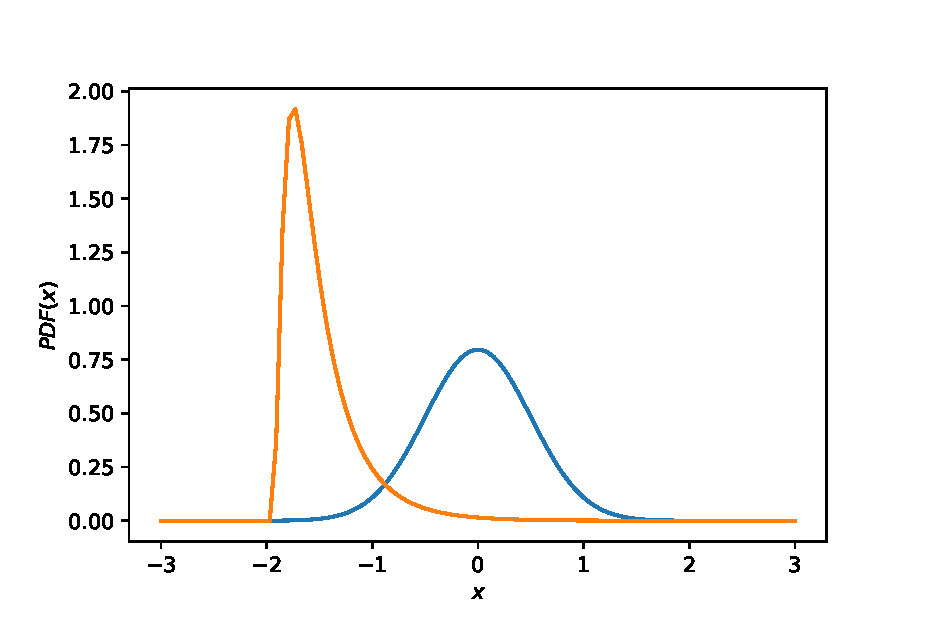
\includegraphics[width=0.5\textwidth]{images/diff-kl-2}}
    \caption{On the left plot the probability density function of two close distributions, the opposite on the right plot.}
    \label{fig:diffkl}
\end{figure}

\section{Kullback–Leibler divergence}
Given two probability distributions $p(x)$ and $q(x)$, we define the KL divergence as:
$$ \mathit{KL}(p \| q) = \int_x p(x) \log_2 \frac{p(x)}{q(x)} = \E_{X \sim p}{[\log_2 \frac{p(x)}{q(x)}]}$$

If the two distributions are discrete, it can be rewritten as:
$$ \mathit{KL}(p \| q) = \sum_i p(i) \log_2 \frac{p(i)}{q(i)}$$

Suppose we have two Categorical distributions $c_1$ and $c_2$ with parameters $p_{c_1} = (0.1, 0.2, 0.7)$ and $p_{c_2} = (0.3, 0.5, 0.2)$, respectively.

Given the formula presented above, we can compute the KL divergence:
\begin{itemize}
    \item $\mathit{KL}(c_1 \| c_2) = 0.1 \log_2 \frac{0.1}{0.3} + 0.2 \log_2 \frac{0.2}{0.5} + 0.7 \log_2 \frac{0.7}{0.2} \approx 0.85$
    \item $\mathit{KL}(c_2 \| c_1) = 0.3 \log_2 \frac{0.3}{0.1} + 0.5 \log_2 \frac{0.5}{0.2} + 0.2 \log_2 \frac{0.2}{0.7} \approx 0.77$
\end{itemize}


\subsection{Proprieties}
From the previous example, it can be seen that the KL divergence is not symmetric: $\mathit{KL}(p \| q) \neq \mathit{KL}(q \| p)$.

Also, note that $\mathit{KL}(p \| p) = \int_x p(x) \log_2 \frac{p(x)}{p(x)} = \int_x p(x) \log_2 (1) = \int_x p(x) \cdot 0 = 0$
and $\mathit{KL}(p \| q) \geq 0$.

\section{Hellinger distance}
The Hellinger distance has some advantages over the Kullback–Leibler divergence:
\begin{itemize}
    \item it is symmetric: $\mathit{HD}(p, q) = \mathit{HD}(q, p)$
    \item it has an upper bound: $0 \leq \mathit{HD}(p, q) \leq 1$
\end{itemize}

Given two discrete probability distributions $p$ and $q$, the Hellinger distance is defined as:
$$\mathit{HD}(p, q) = \mathit{HD}(q, p) = \frac{1}{\sqrt{2}} \sqrt{\sum_i (\sqrt{p(i)} - \sqrt{q(i)})^2}$$
Note that in the literature the Hellinger distance is defined in different ways (e.g. with or without $\frac{1}{\sqrt{2}}$).

\section{References}
The interested reader may refer to \cite{Joyce2011} and \cite{Hellinger1909} for further analysis of the topic.
\chapter{Variational Inference} \label{vi}
Variational inference is a method that approximates probability densities through optimization.

Denoting $x$ as the observations and $z$ as the hidden variables,
we want to compute the posterior distribution $p(z | x)$.

In particular, we want to find a $q(z | v)$ over a family of densities
which is as similar as possible to $p(z | x)$ using the Kullback–Leibler divergence as a measure of closeness:
\begin{equation} \label{eq:klexpanded}
    \begin{split}
        KL(q || p) & = \E_q {[\log_2 \frac{q(z | v)}{p(z | x)}]} \\
        & = \E_q \log_2 [q(z | v)] - \E_q \log_2 [p(z | x)] \\
        & = \E_q \log_2 [q(z | v)] - \E_q \log_2 [\frac{p(z,x)}{p(x)}] \\
        & = \E_q \log_2 [q(z | v)] - \{ \E_q \log_2 [p(z,x)] - \E_q \log_2 [p(x)] \} \\
        & = \E_q \log_2 [q(z | v)] - \{ \E_q \log_2 [p(z,x)] - \log_2 [p(x)] \} \\
        & = \E_q \log_2 [q(z | v)] - \E_q \log_2 [p(z,x)] + \log_2 [p(x)]
    \end{split}
\end{equation}
Note that $q(z | v)$ does not depend on the observed data.

To do so, we start by computing $p(x)$:
\begin{equation*}
    \begin{split}
        p(x) & = \log_2[p(x)] \\
        & = \log_2[\int p(x,z) dz]  \\
        & = \log_2[\int \frac{q(z | v)}{q(z | v)} p(x,z) dz] = \log_2[\int q(z | v) \frac{p(x,z)}{q(z | v)} dz] \\
        & = \log_2[\E_q \frac{p(x,z)}{q(z | v)}]
    \end{split}
\end{equation*}

The Jensen's inequality says that if a function $f$ is concave, $f(\E[x]) \geq \E[f(x)]$.
Since the logarithm is a concave function, we can state that:
$$ \log_2[\E_q \frac{p(x,z)}{q(z | v)}] \geq \E_q \log_2[\frac{p(x,z)}{q(z | v)}] $$
$$ \log_2[\E_q \frac{p(x,z)}{q(z | v)}] \geq \E_q log_2[p(x,z)] - \E_q log_2[q(z | v)] $$

Given that $ \displaystyle \E_q \{log_2[p(x,z)] - log_2[q(z | v)]\} = - E_q \{ log_2[p(x,z)] -log_2[q(z | v)]) \}$
and the fact that $\log_2[p(x)]$ is a constant that does not depend on $q$,
maximizing the lower bound of $p(x)$ is equivalent to minimizing the Kullback–Leibler divergence between $q$ and $p$ (see Equation \ref{eq:klexpanded} to a comparison).
From now, we refer to this lower bound as ELBO.

\section{Mean field variational inference}
In order to have a tractable problem, these distributions must have the characteristic
of removing the mutual dependence between the hidden variables:
$$ q(z_1, ..., z_m| v) = \prod_{j=1}^m q(z_j | v_j) $$

Since we want to maximize ELBO,
the final step for obtaining a solution is to take the partial derivatives of it and set them equal to zero.
Then, we solve the problem iteratively for each variable of interest using coordinate-ascent optimization until convergence.
Note that the algorithm converges to a local maximum and not a global one.

\section{References}
The interested reader is advised to read \cite{Blei_2017} in conjunction with this in order to have an overall idea of the topic.

\bibliographystyle{alphaurl}
\bibliography{bib}

\chapter*{License}
\begin{center}
    \includegraphics{images/cc.eps}

    This work by \url{https://github.com/Davide95/msc_thesis/tree/master/thesis} is licensed under a \linebreak
    \href{https://creativecommons.org/licenses/by-sa/4.0/}{Creative Commons Attribution-ShareAlike 4.0 International License}.
\end{center}

\end{document}

